% imports
\documentclass[titlepage]{article}
\usepackage{graphicx} % Required for inserting images
\usepackage[colorlinks=true, urlcolor=blue]{hyperref}
\usepackage{titlepic}
\usepackage{geometry}
\usepackage[section]{placeins}

\graphicspath{{./assets/}}

% formatting
\geometry{margin=1in}

% Title items
\titlepic{
\includegraphics[scale=0.4]{assets/cisess.png}}
\title{\huge CISESS Technical Report}
\author{
\href{mailto:huyang@umd.edu}{Hu Yang},
\href{mailto:nho08@umd.edu}{Nathan Ho}
}
\date{June 2024 - August 2024}


% Start of report
\begin{document}


% Title
\begin{titlepage}    
    \maketitle
\end{titlepage}


% Introduction
\section{Introduction: Project Overview}
\label{introduction}

Water vapor content in the atmosphere contains important information and is commonly used to predict ground-level weather conditions. Vapor levels can be sampled by emitting microwaves and collecting their reflections - the power of the reflection can indicate certain qualities in the atmosphere that dictate precipitation, temperature, and other information. A tool that does this is called a microwave radiometer. Currently, CISESS has a low-cost microwave radiometer, however it is limited largely by its internal clock and ADC chip, which limit the data resolution and data sampling rate. The goal this year is to transfer the back-end signal processing system from Arduino microprocessors to a \href{https://digilent.com/reference/programmable-logic/arty-s7/start}{Digilent Arty S7 Spartan} FPGA board as a proof of concept for future FPGA design regarding this project. The FPGA boasts a faster internal clock, as well as a more powerful Analog-Digital Conversion (ADC) chip, which should lead to a higher output data resolution.

\begin{figure}[h]
    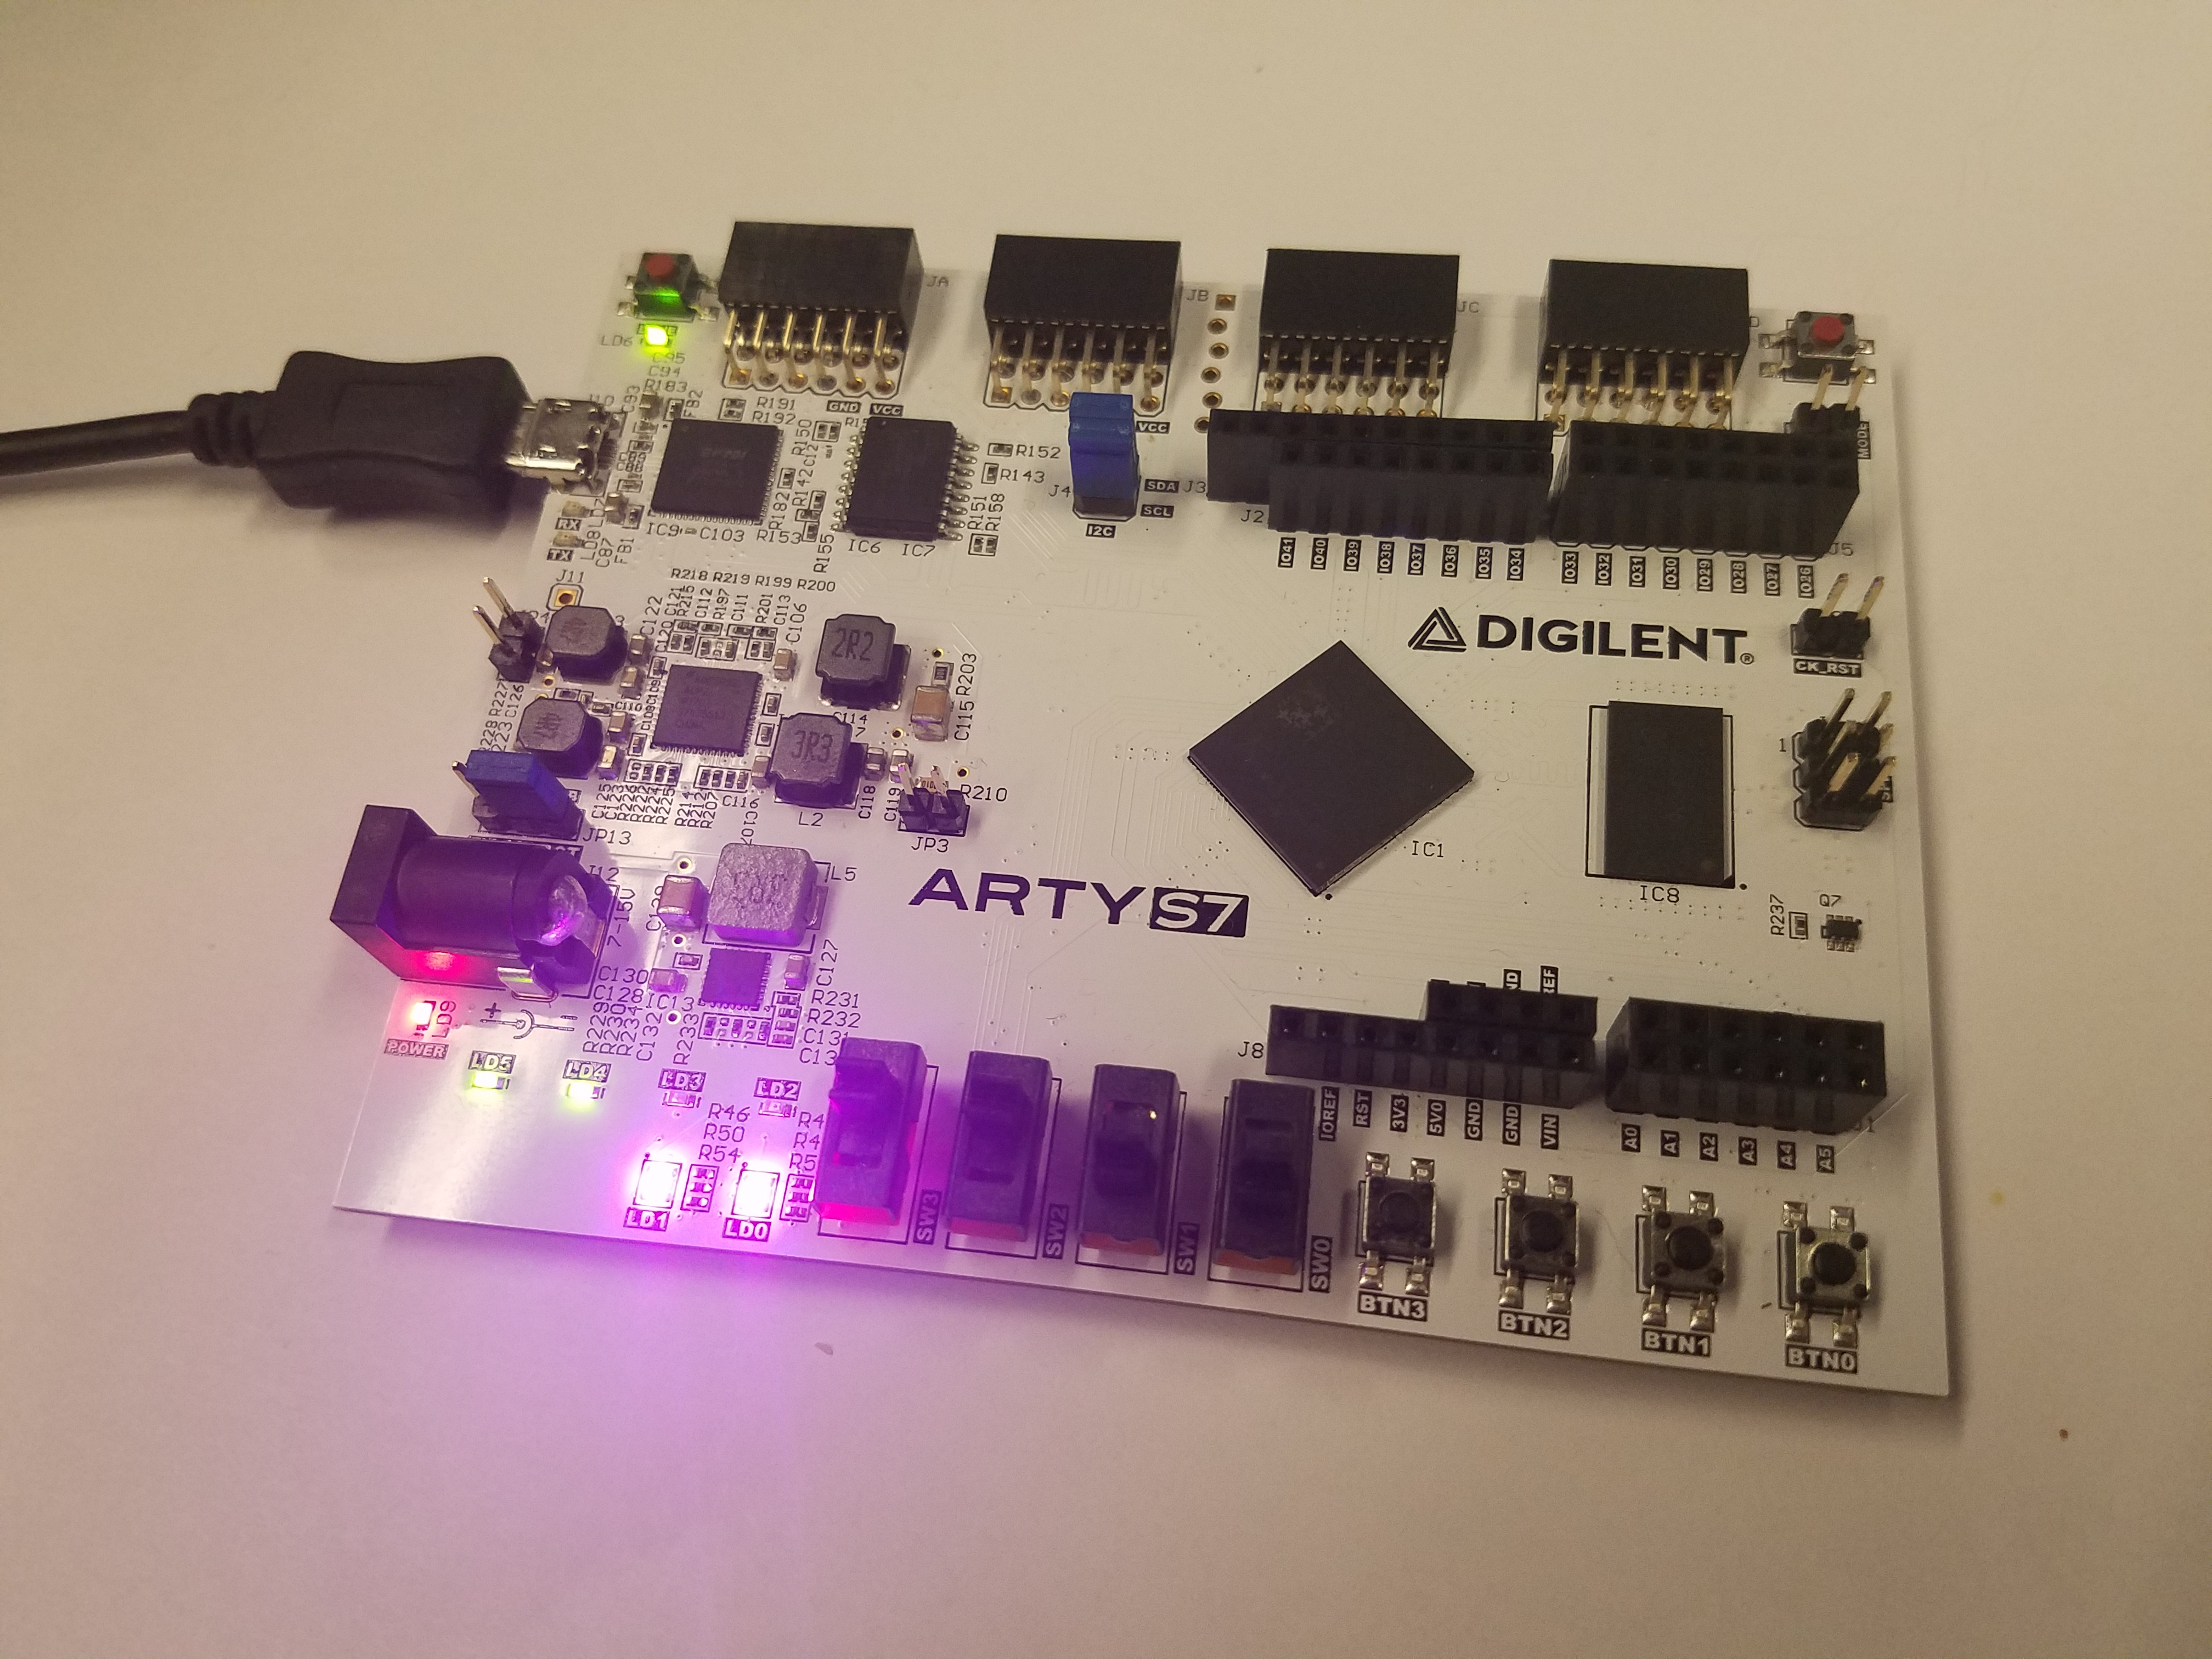
\includegraphics[width=\textwidth]{assets/arty.jpg}
    \centering
    \caption{Digilent Arty S7 FPGA board}
\end{figure}
\label{figure1}


\section{Instrument Description}
\label{instrunment description}

The microwave radiometer works as follows: 22GHz reflections are first detected by a feed horn. The RF signal is sampled by a switch which is controlled by a PWM signal generated by the back-end signal processing system to limit the sample rate. The samples that pass through are routed to an LNB (Low Noise Block Down-converter) to amplify and down-convert the frequency of the signal. Finally, the signal passes through a power converter to convert RF power into DC voltage and then to the back-end signal processing whose job it is to reconstruct the signal.

\newpage

\begin{figure}[h]
    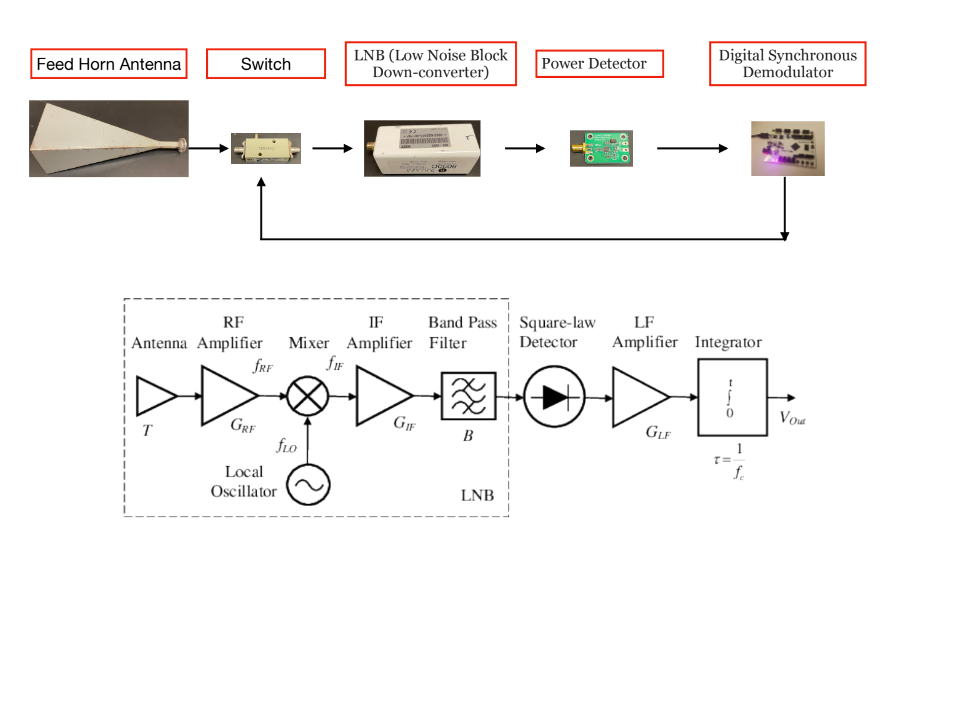
\includegraphics[width=\textwidth]{assets/flow_chart.png}
    \centering
    \caption{Visual and block diagrams of signal processing system}
\end{figure}
\label{figure2}

\noindent
From here on, the ``back-end signal processing", will be referred to as the `Digital Synchronous Demodulator'.


\section{Digital Synchronous Demodulator}
\label{digital synchronous demodulator}

The signal processing system has 2 main tasks:
\begin{itemize}
    \item[i.] Produce the switch control PWM signal
    \item[ii.] Handle the demodulation of the feed signal
\end{itemize}
To complete these tasks, the system is split into 2 sections, taking advantage of Verilog's hierarchy system.


\subsection{Switch Control}
\label{DSD switch control}

The switch control module will output the driver signal for the switch. The PMOD ports will be used to output the signal.


\subsection{Demodulation}
\label{DSD demod}

The input signal contains two main components: one referred to as the ``scene signal" (water vapor data), and noise from the environment. In order to remove this noise and preserve the scene signal, the feed horn input will be sampled at points when the switch is open (noise) or closed (noise and scene), and a difference will be taken between these samples. To do this, in addition to being output, the switch PWM signal will also be routed internally to the ADC module, where the FPGA can use it as a clock. If the signal is high then we know that the switch is closed, and if open, vise-versa. Therefore, all that's left to do is subtract. What remains after subtraction is the demodulated water vapor data for that period.

\subsection{Implementation}
\label{DSD implementation overview}

For this implementation, the AMD Vivado Design Suite was used to synthesize RTL logic with Verilog HDL. The following code assumes a basic understanding of Verilog and its syntax and semantics. Not pictured in this report is the top-level module that was used to combine all these sub-modules under a singular hierarchy for synthesis (you can find that, as well as the raw, downloadable HDL \href{https://github.com/ptrichr/CISESS-2024/tree/main}{here}).


\subsubsection{Switch Control Module}
\label{DSD switch control implementation}
\small
\begin{verbatim}
module switch_controller (
input                clk,
output  reg          pwm
);

integer count;

initial begin
    count = 0;
end

// factor of 48000 downscales 100MHz to 2.083KHz
always @(posedge clk) 
begin
    // up time
    if (count < 23999)
    begin
        pwm <= 1;
        count <= count + 1;
    end
    // down time
    else 
    begin
        if (count < 47999) 
        begin
            pwm <= 0;
            count <= count + 1;
        end
        // reset
        else 
        begin
            pwm <= 1;
            count <= 0;
        end
    end
end 

endmodule
\end{verbatim}
\normalsize
\noindent
Above is the code used to synthesize the RTL logic for a 2.083KHz square wave signal, which controls the switch responsible for sampling the input signal. It operates as a basic clock divider, scaling down the 100MHz system clock by a factor of 48000 to drive the switch.


\subsubsection{ADC Clock}
\label{DSD ADC clk}
\small
\begin{verbatim}
module adc_clock_divider (
input           clk         ,
output  reg     clk_enable
);

integer count;

initial begin
    count = 0;
end

// factor of 3000 downscales 100MHz to 33.33KHz
always @(posedge clk) 
begin
    // up time
    if (count < 1499)
    begin
        clk_enable <= 1;
        count <= count + 1;
    
    end
    // down time 
    else 
    begin
        if (count < 2999) 
        begin
            clk_enable <= 0;
            count <= count + 1;
        end
        // reset
        else 
        begin
            clk_enable <= 1;
            count <= 0;
        end
    end
end

endmodule
\end{verbatim}
\normalsize
This module divides the system clock from 100MHz to 33.33KHz, which is the correct frequency for the ADC.


\subsubsection{ADC Module}
\label{DSD ADC}
\small
\begin{verbatim}
module adc (
input               clk             ,       // System clock
input               switch_pwm      ,       // switching PWM
input               feed_signal     ,       // B13 (A0 on board)
input               feed_ground     ,
output reg  [3:0]   LED             ,       // LED for testing
output reg  [11:0]  denoise                 // Denoise data
);


// ADC variables
wire enable;  
wire ready;
reg ready_d1;
wire ready_rising;
wire ready_falling;
wire [15:0] data;               // the 12 most significant bits store ADC data
reg [6:0] Address_in;

// Storing data for demodulation
integer on_data;
integer off_data;
reg on_ready;
reg off_ready;


//-----------------------------------------------------------------------------
// clock divider for ADC 100MHz -> 33.33kHz
wire clk_en;

adc_clock_divider
d(
.clk            (clk            ),
.clk_enable     (clk_en         )
);


//-----------------------------------------------------------------------------
// xadc instantiation connect the eoc_out .den_in to get continuous conversion
// xadc dclk needs the system clock (100MHz)
xadc_wiz_0 xadc
(
    .daddr_in(8'h10),                   // Address bus for the dynamic reconfiguration port
    .dclk_in(clk),                      // Clock input for the dynamic reconfiguration port
    .den_in(enable),                    // Enable Signal for the dynamic reconfiguration port
    .di_in(0),                          // Input data bus for the dynamic reconfiguration port
    .dwe_in(0),                         // Write Enable for the dynamic reconfiguration port
    .reset_in(0),                       // Reset signal for the System Monitor control logic
    .busy_out(),                        // ADC Busy signal
    .channel_out(),                     // Channel Selection Outputs
    .do_out(data),                      // Output data bus for dynamic reconfiguration port
    .eoc_out(enable),                   // End of Conversion Signal
    .eos_out(),                         // End of Sequence Signal
    .alarm_out(),                       // OR'ed output of all the Alarms  
    .drdy_out(ready),                   // Data ready signal for the dynamic reconfiguration port
    
    .vp_in(),
    .vn_in(),
    .vauxp0(feed_signal),
    .vauxn0(feed_ground)
);


//-----------------------------------------------------------------------------
// driver signals for XADC IP
always @(posedge clk_en)
begin
    ready_d1 <= ready;
end


assign ready_rising = ready && !ready_d1 ? 1'b1 : 1'b0;
assign ready_falling = !ready && ready_d1 ? 1'b1 : 1'b0;

[...]
\end{verbatim}
\normalsize
The first part of this module (the above), deals with instantiating the XADC IP core and the clock divider that was mentioned in the previous subsection of this report (\ref{DSD ADC clk}). This \href{https://github.com/Digilent/Arty-S7-50-XADC}{demo} was used as reference for the IP instance.

\begin{verbatim}
[... continued]

//led visual on board              
always @(posedge clk)
begin
  if (ready_rising == 1)
  begin
      case (data[15:13])
        4: LED <= 4'b0001;
        5: LED <= 4'b0011;
        6: LED <= 4'b0111;
        7: LED <= 4'b1111;
        default: LED <= 6'b0; 
      endcase
  end
  else
      LED <= LED;
end

//-----------------------------------------------------------------------------
// Denoise logic

// collect data from either on or off. if data has been collected from both, reset
always @(posedge clk_en)
begin
    if (on_ready == 1 && off_ready == 1)
    begin
        on_ready <= 0;
        off_ready <= 0;
    end

    if (switch_pwm == 1)
    begin
        on_data <= data[15:4];
        on_ready <= 1;
    end
    else
    begin
        off_data <= data[15:4];
        off_ready <= 1;
    end
end

// assign denoise.
always @(*)
begin
    if (on_data > off_data)
        denoise <= on_data - off_data;
    else
        denoise <= 0;           // handles underflow
        
    on_ready <= 0;
    off_ready <= 0;
end


endmodule
\end{verbatim}
\normalsize
This section of the module deals with removing the noise from the signal. It uses the methods described above in the overview of the Digital Synchronous Demodulator (\ref{DSD demod}).

\section{Testing}
\label{testing}

In order to verify the functionality of the upgraded systems, we performed benchmarks with controlled signals. However, to monitor the output we also had to implement a communication protocol so that the demodulation data can be viewed. The UART protocol was deemed a simple - yet effective - method to serialize and display our data on an external device, for the purpose of testing.

\subsection{UART Module}
\label{testing uart}
\small
\begin{verbatim}
module uart_tx (
input  wire     clk             ,       // 100 MHz clock input
input  wire     reset           ,       // Reset
input  wire     [11:0] data     ,       // 12-bit data input
input  wire     start           ,       // Start transmission signal
output reg      uart_txd        ,       // UART TXD pin
output reg      busy                    // Busy
);

// Baud rate calculation
localparam BAUD_RATE = 115200;
localparam CLOCK_FREQ = 100_000_000;
localparam BAUD_COUNTER_MAX = CLOCK_FREQ / BAUD_RATE;

// UART state machine states
localparam IDLE = 3'b000,
           START1 = 3'b001,
           DATA1 = 3'b010,
           STOP1 = 3'b011,
           NEXT = 3'b100,
           START2 = 3'b101,
           DATA2 = 3'b110,
           STOP2 = 3'b111;

reg [2:0] present_state, next_state;

// Counter for baud rate
reg [15:0] baud_counter;

// reg to hold data halves, bit counter to keep position
reg [7:0] byte1, byte2;
reg [3:0] bit_counter;

// split demod data into 2 bytes
always @(posedge clk or posedge reset)
begin
    if (reset)
    begin
        byte1 <= 8'b0;
        byte2 <= 8'b0;
    end
    else if (start)
    begin
        byte1 <= {4'b0000, data[11:8]}; // 4 MSBs padded with 4 zeros
        byte2 <= data[7:0];             // 8 LSBs
    end
end

// FSM
always @(posedge clk or posedge reset)
begin
    if (reset)                          // idle when reset is enabled
    begin
        present_state <= IDLE;
        baud_counter <= 0;
        bit_counter <= 0;
        uart_txd <= 1'b1;
        busy <= 1'b0;
    end
    else                                // normal output logic
    begin
        present_state <= next_state;
        case (present_state)
            IDLE:
            begin
                uart_txd <= 1'b1;
                if (start)
                begin
                    busy <= 1'b1;
                    next_state <= START1;
                end
                else
                begin
                    busy <= 1'b0;
                end
            end

            START1:
            begin
                if (baud_counter == BAUD_COUNTER_MAX)
                begin
                    uart_txd <= 1'b0; // Start bit
                    baud_counter <= 0;
                    bit_counter <= 0;
                    next_state <= DATA1;
                end
                else
                begin
                    baud_counter <= baud_counter + 1;
                end
            end

            DATA1:
            begin
                if (baud_counter == BAUD_COUNTER_MAX)
                begin
                    baud_counter <= 0;
                    uart_txd <= byte1[bit_counter]; // Send bits of byte1
                    bit_counter <= bit_counter + 1;
                    if (bit_counter == 7) begin
                        next_state <= STOP1;
                    end
                end
                else
                begin
                    baud_counter <= baud_counter + 1;
                end
            end

            STOP1:
            begin
                if (baud_counter == BAUD_COUNTER_MAX)
                begin
                    uart_txd <= 1'b1; // Stop bit
                    baud_counter <= 0;
                    next_state <= NEXT;
                end
                else
                begin
                    baud_counter <= baud_counter + 1;
                end
            end

            NEXT:
            begin
                if (baud_counter == BAUD_COUNTER_MAX)
                begin
                    uart_txd <= 1'b0; // Start bit for next byte
                    baud_counter <= 0;
                    bit_counter <= 0;
                    next_state <= DATA2;
                end
                else
                begin
                    baud_counter <= baud_counter + 1;
                end
            end

            DATA2:
            begin
                if (baud_counter == BAUD_COUNTER_MAX)
                begin
                    baud_counter <= 0;
                    uart_txd <= byte2[bit_counter]; // Send bits of byte2
                    bit_counter <= bit_counter + 1;
                    if (bit_counter == 7) begin
                        next_state <= STOP2;
                    end
                end
                else
                begin
                    baud_counter <= baud_counter + 1;
                end
            end
            STOP2:
            begin
                if (baud_counter == BAUD_COUNTER_MAX)
                begin
                    uart_txd <= 1'b1; // Stop bit
                    baud_counter <= 0;
                    busy <= 1'b0;
                    next_state <= IDLE;
                end
                else
                begin
                    baud_counter <= baud_counter + 1;
                end
            end
        endcase
    end
end

endmodule
\end{verbatim}
\normalsize
Simple UART implementation adjusted for transmitting 2 consecutive bytes of data.


\subsection{Procedure}
\label{testing procedure}
The following section will cover the in-lab testing procedure for these modules.

\begin{itemize}
    \item Switch Control Module: The switch control module output was directly tested with an oscilloscope for the specified output frequency.
    \item ADC Module: The ADC module was tested by sampling a known signal from a signal generator. The output of the ADC via serial terminal was then graphed to determine whether or not there was a correlation with the original signal.
\end{itemize}


\subsection{Results}
\label{testing results}
Both modules met their expectations for functionality during testing. The figures showcased in the following pages showcase testing apparatus as well as the information that was used to verify functionality. 

\newpage

\begin{figure}[h]
    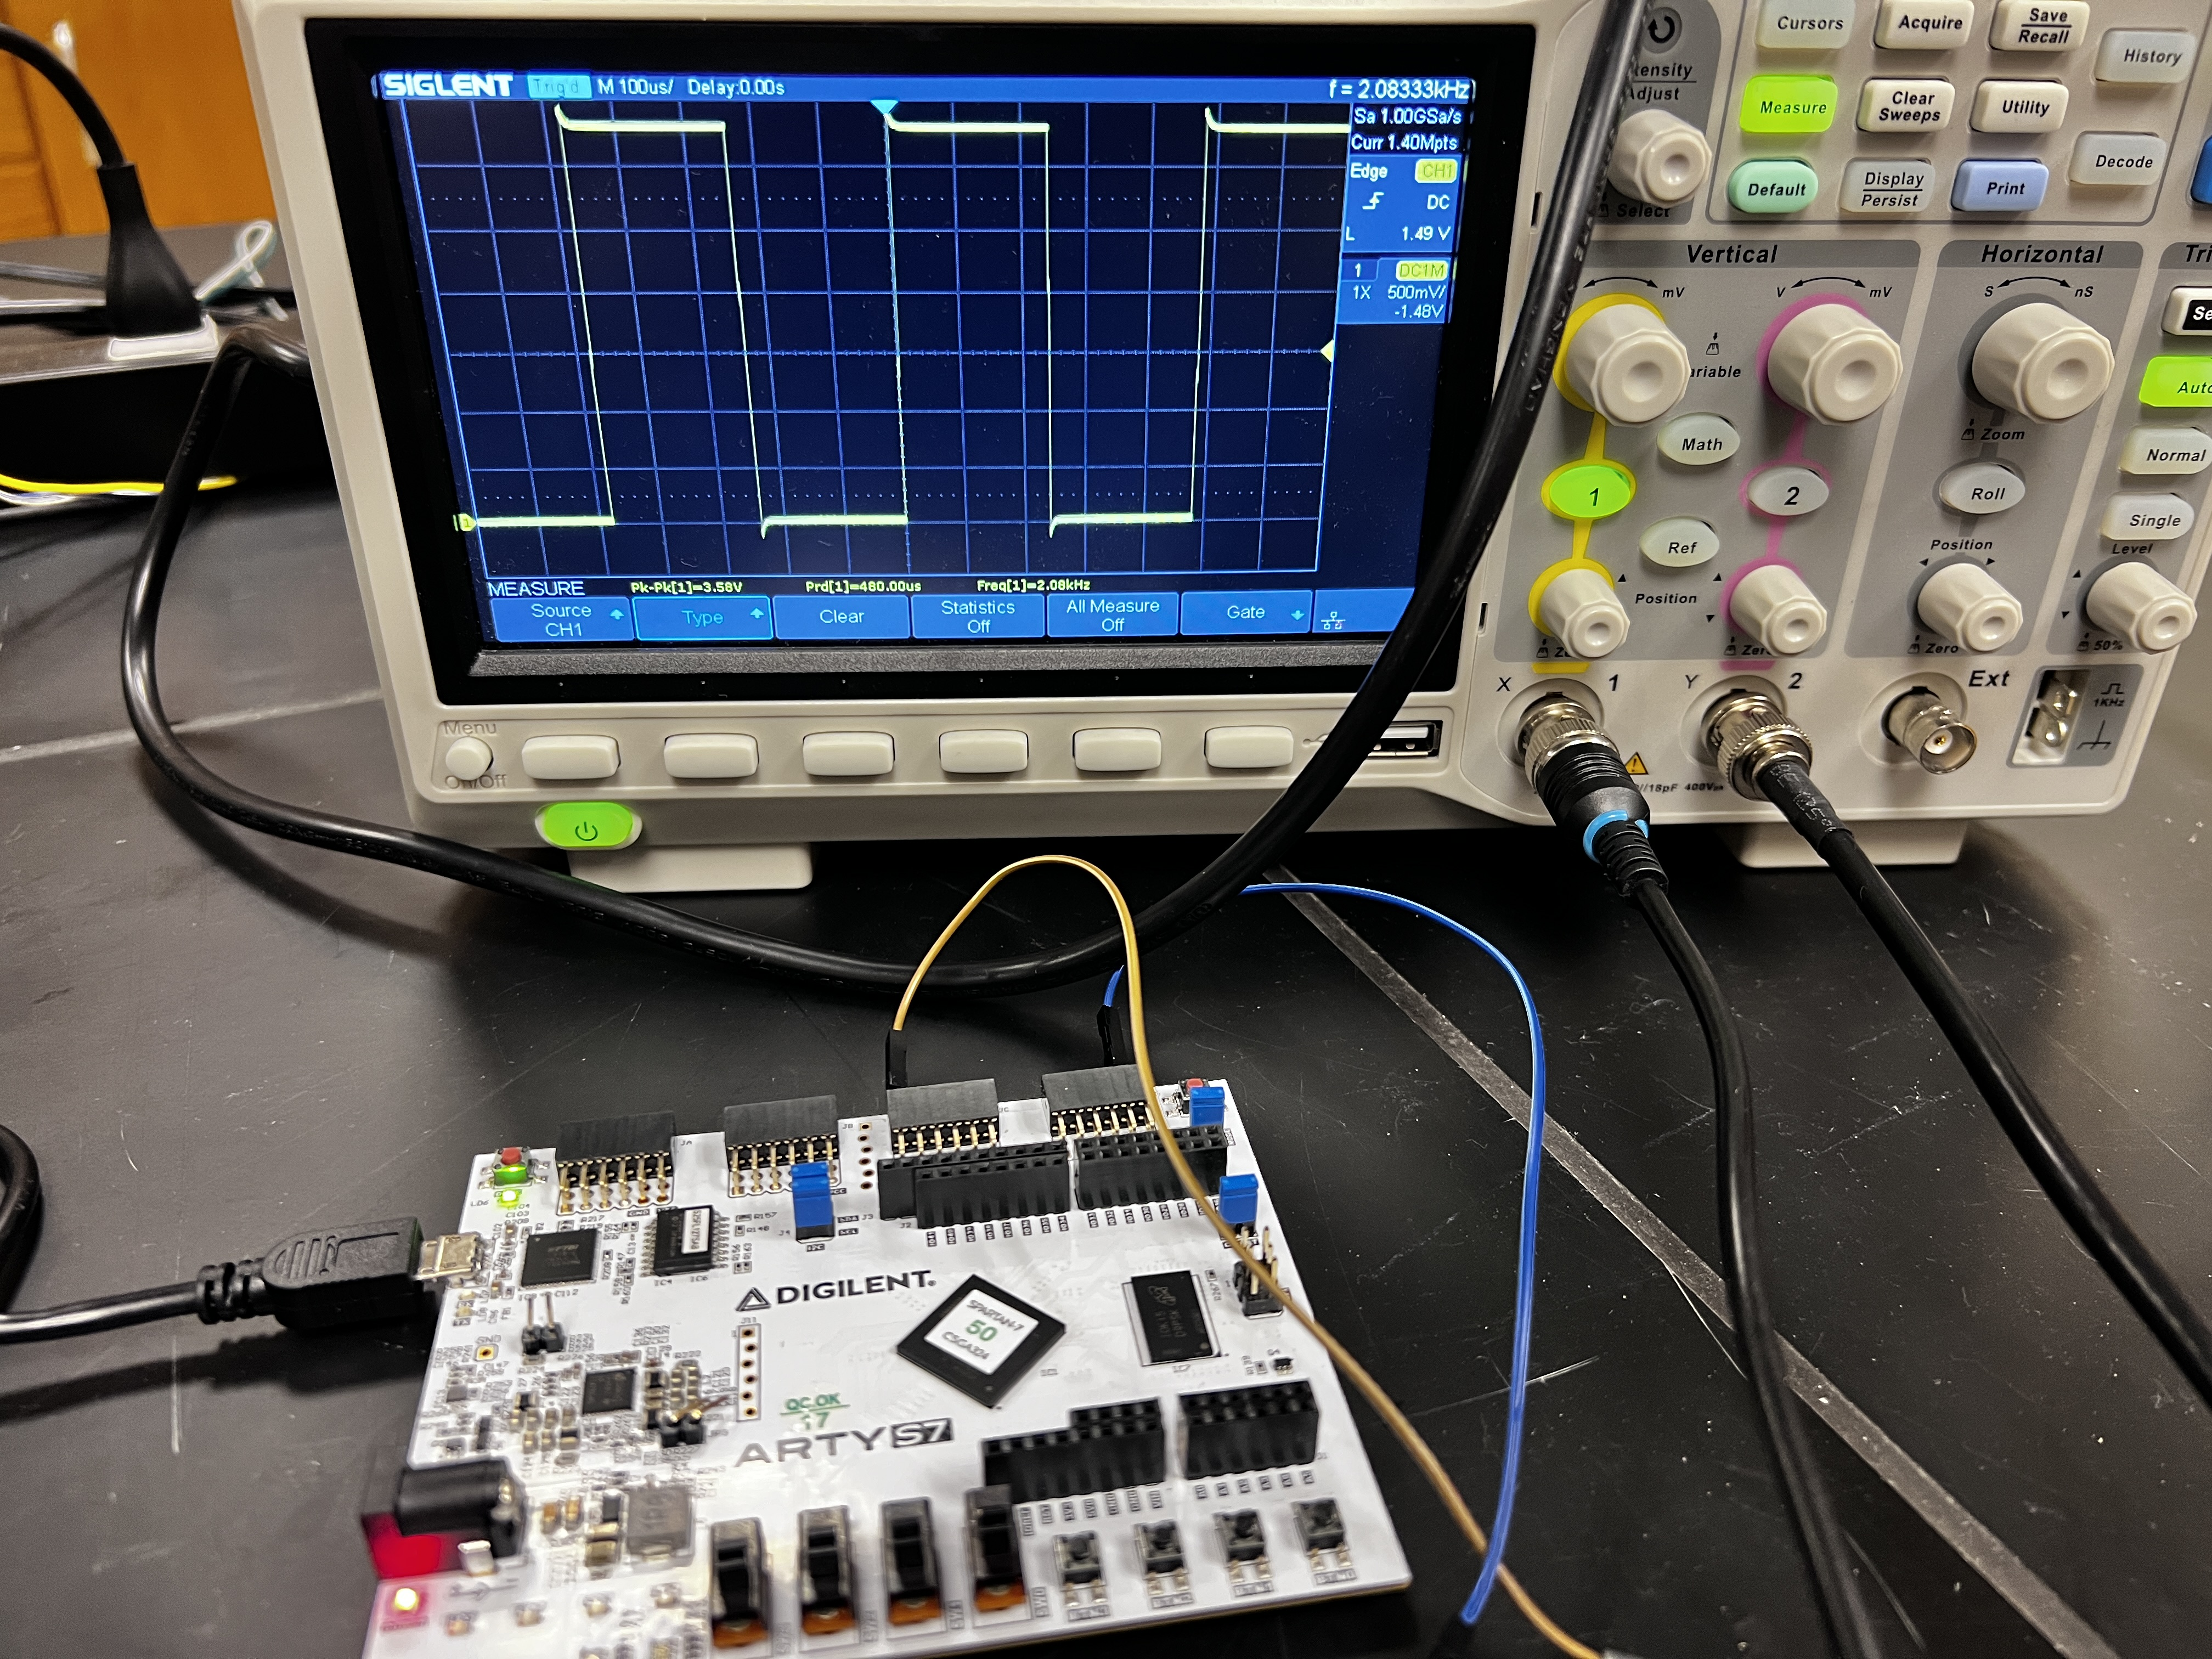
\includegraphics[width=\textwidth]{assets/pwmtest.jpg}
    \centering
    \caption{Testing setup and results for the switch control module}
\end{figure}
\label{figure3}

\noindent
The frequency measured in the output waveform by the oscilloscope is exactly the frequency specified for the function of the switch control module. This verifies the functionality of the switch control module.

\newpage

\begin{figure}[h]
    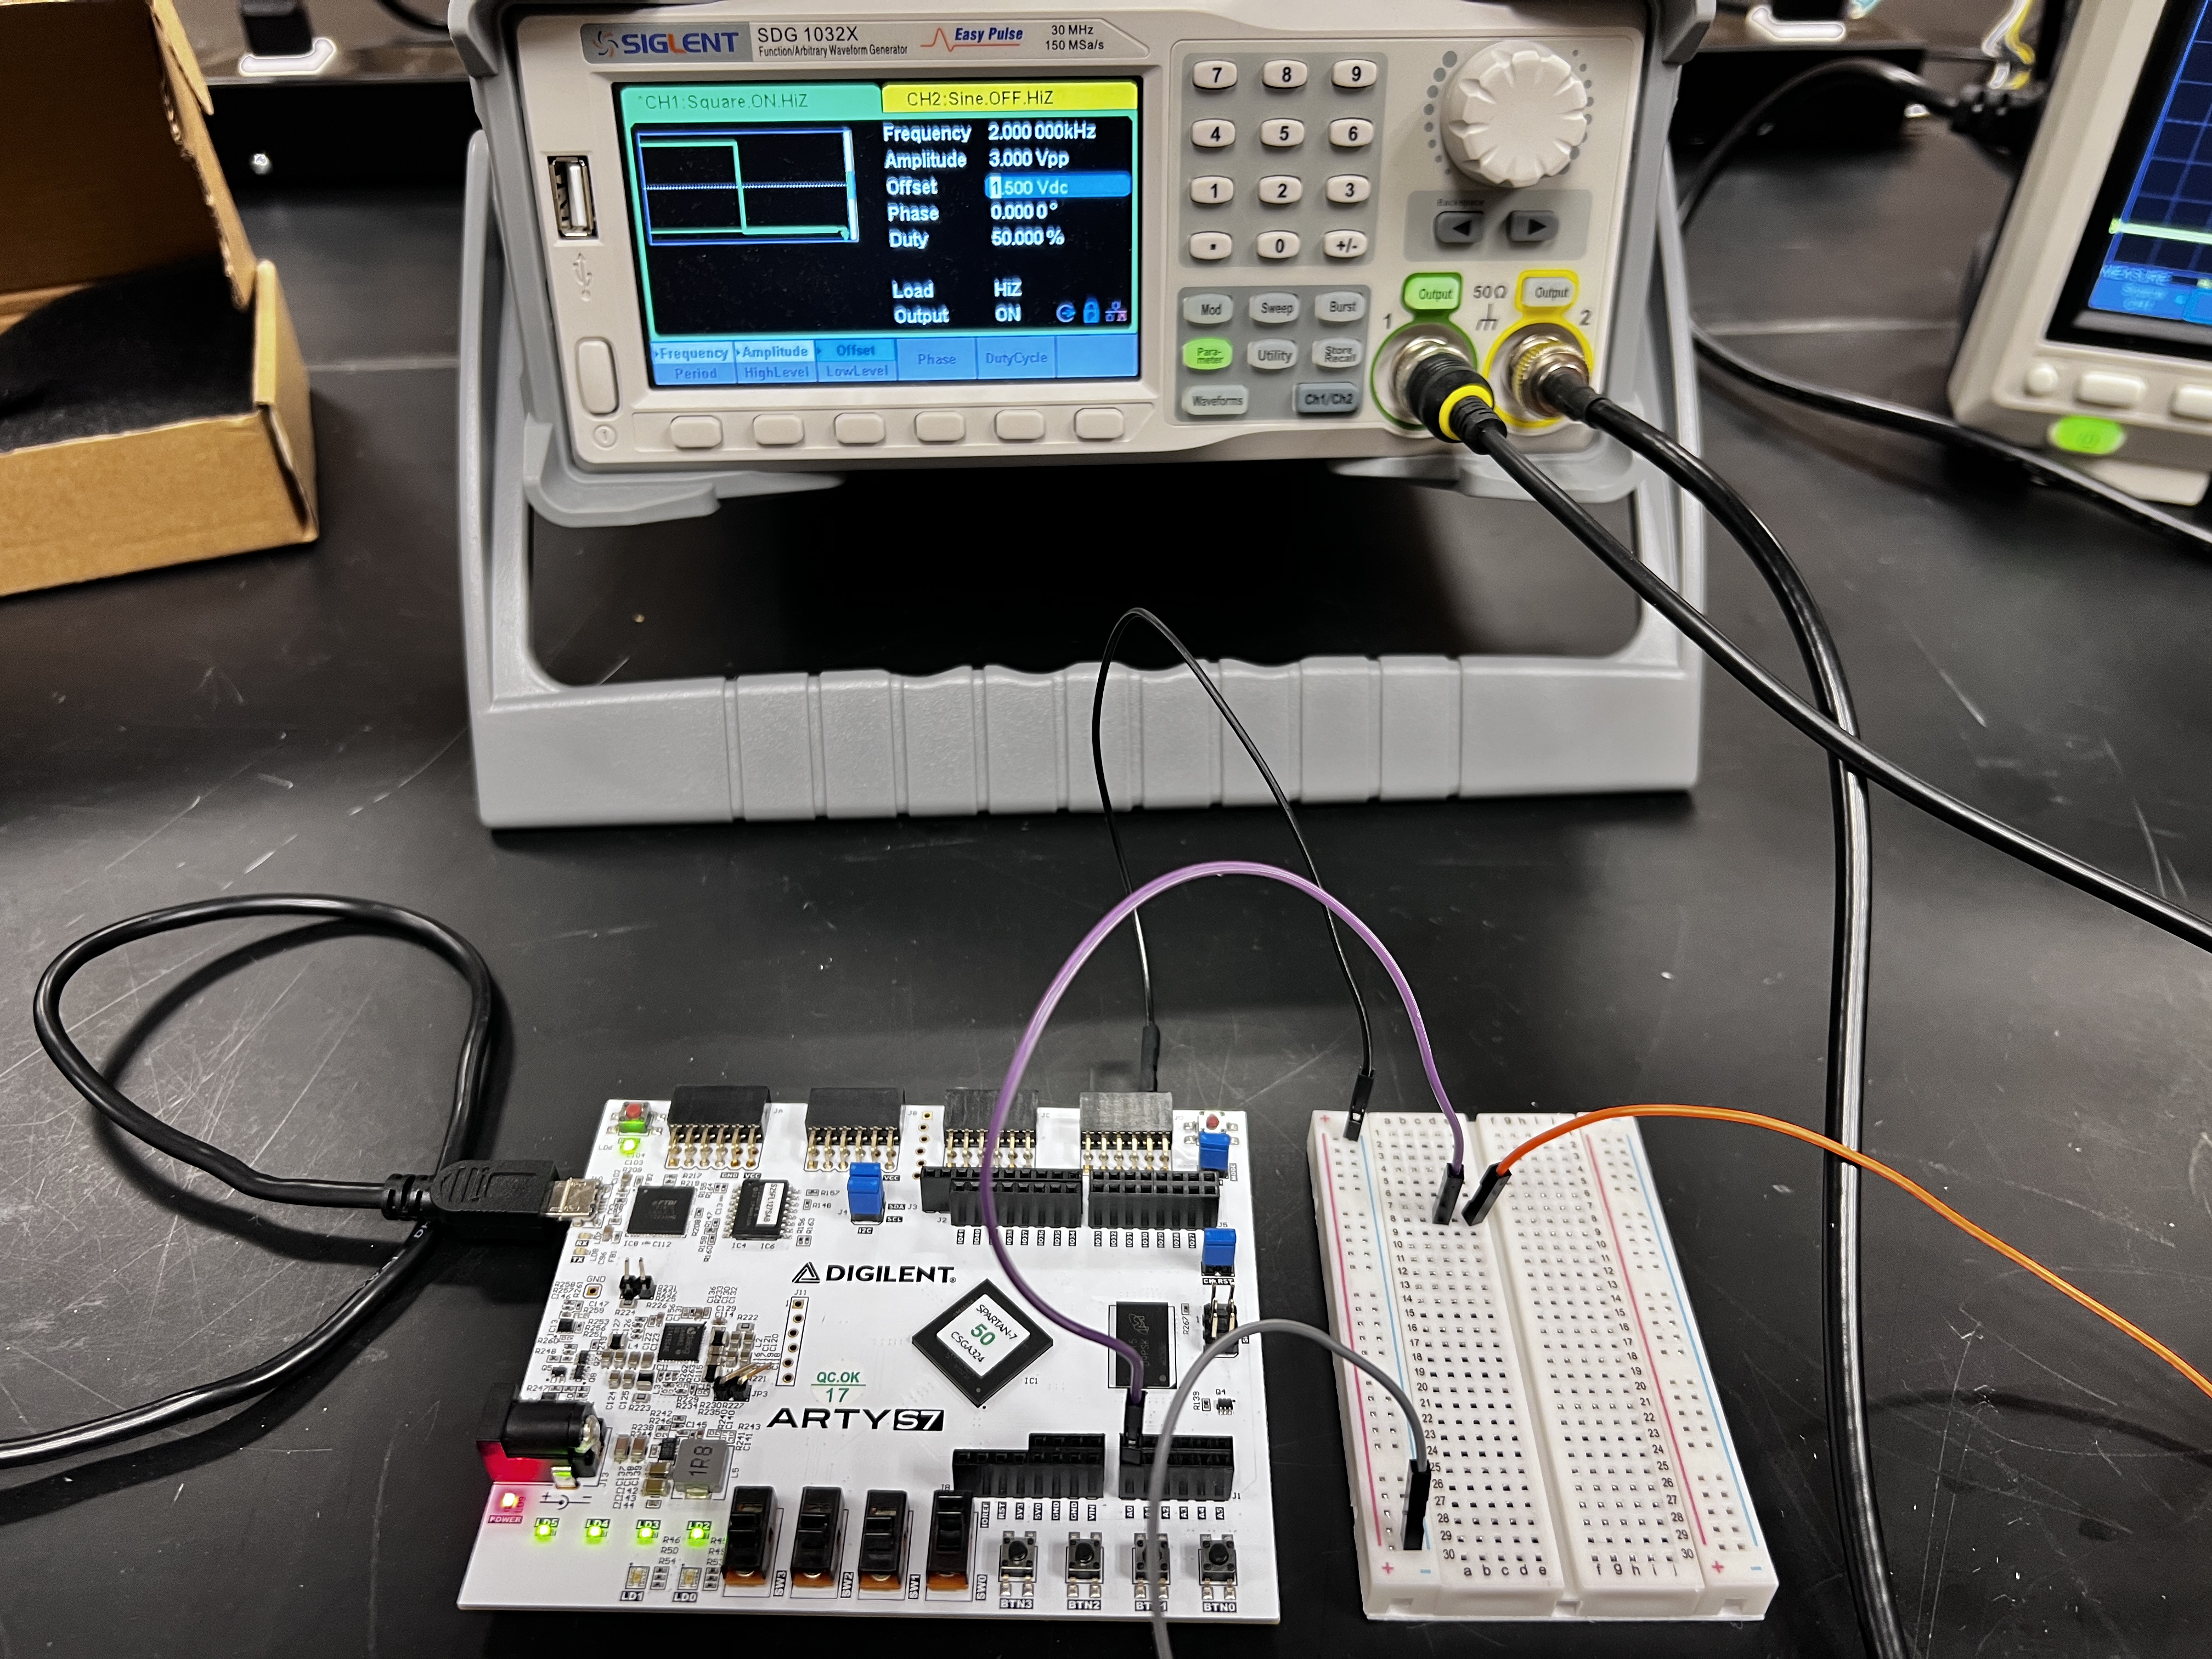
\includegraphics[width=0.78\textwidth]{assets/adctest.jpg}
    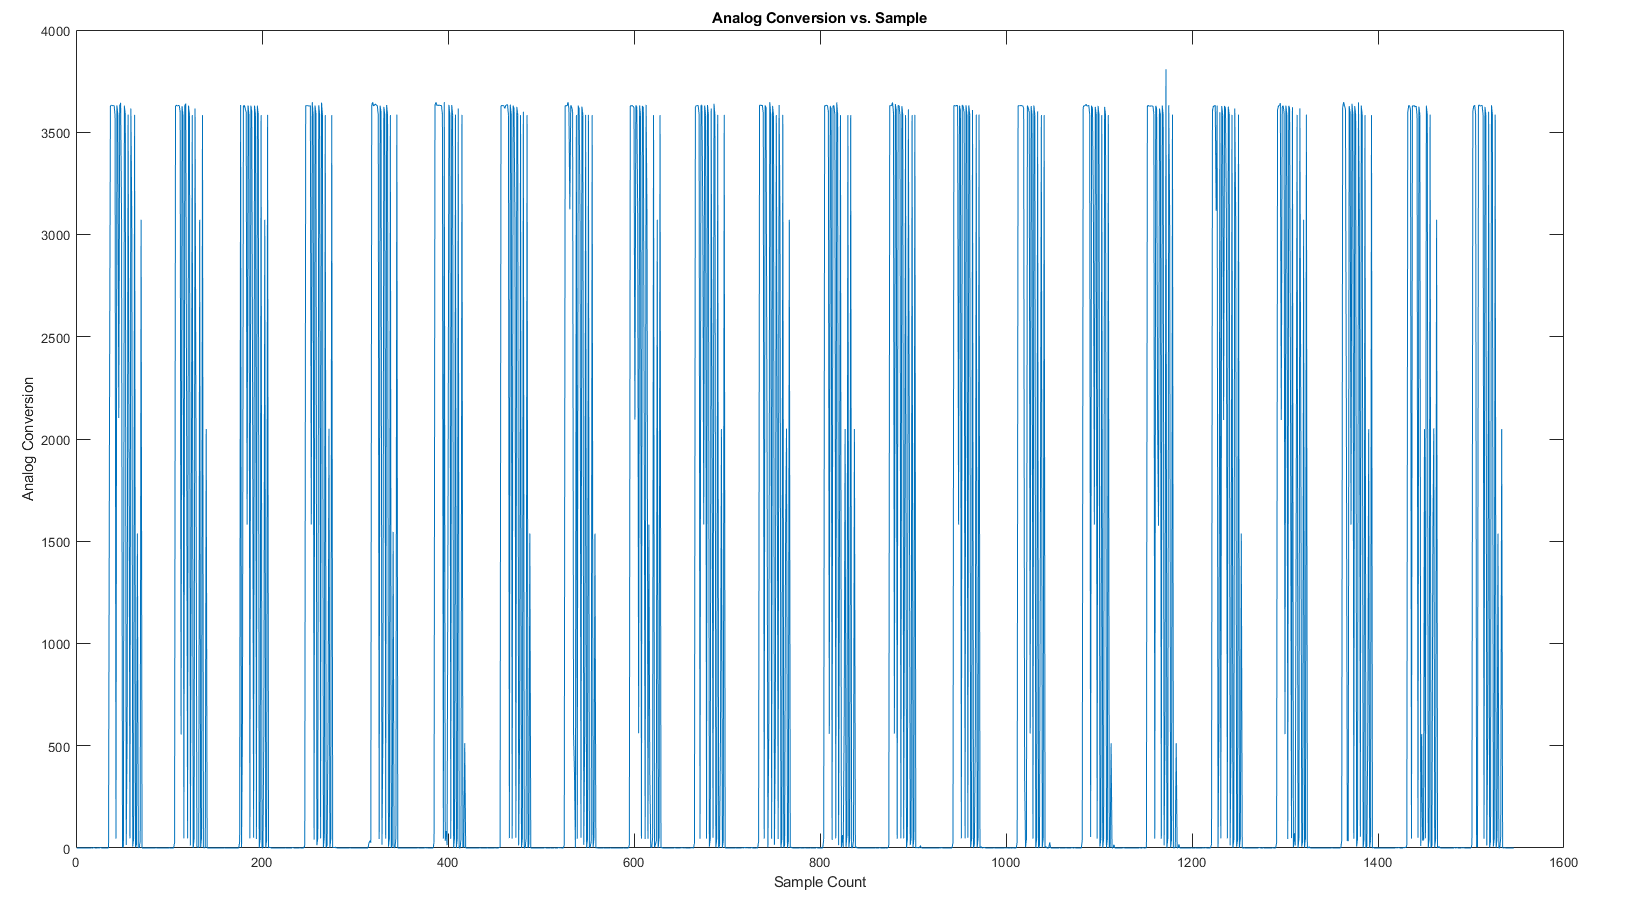
\includegraphics[width=0.78\textwidth]{assets/adcfigure.png}
    \centering
    \caption{Testing setup and results for the ADC module}
\end{figure}
\label{figure4}

\noindent
The setup shows that the signal generator is outputting a square wave with a 50\% duty cycle. The graph in the figure represents the output of the ADC module plotted in MATLAB. The resulting waveform represents a 50\% duty cycle square wave, consistent over a number of cycles. This verifies the functionality of the ADC module.


\newpage

\section{Conclusion}
\label{conclusion}
This project serves as a proof of concept for using FPGA-based design to control and process data within a microwave radiometer system. Since this design is modular, in the future, more modules can be added for further data processing, such as FFT. There is also still room for improvement with sampling frequencies, as 33KHz is still slow relative to the system clock - although a problem this presents is a method to capture the data fast enough to not cause a bottle neck, which is another point to improve on.


\section{References}
\label{references}
\begin{itemize}
    \item[1.] \href{https://digilent.com/reference/_media/reference/programmable-logic/arty-s7/arty_s7_sch-rev_e.pdf?_ga=2.225255450.1624256360.1717423047-1076205636.1717423047}{Arty-S7 Schematic}
    \item[2.] \href{https://docs.rs-online.com/06a7/0900766b815f2fe4.pdf}{Arty-S7 User Manual}
    \item[3.] \href{https://github.com/Digilent/Arty-S7-50-XADC}{XADC Demo for Arty S7}
    \item[4.] \href{https://github.com/ben-marshall/uart}{Open-Source UART Transmitter}
    
\end{itemize}

\end{document}
